%iffalse
\let\negmedspace\undefined
\let\negthickspace\undefined
\documentclass[journal,12pt,onecolumn]{IEEEtran}
\usepackage{cite}
\usepackage{amsmath,amssymb,amsfonts,amsthm}
\usepackage{algorithmic}
\usepackage{graphicx}
\usepackage{textcomp}
\usepackage{xcolor}
\usepackage{txfonts}
\usepackage{listings}
\usepackage{enumitem}
\usepackage{mathtools}
\usepackage{gensymb}
\usepackage{comment}
\usepackage[breaklinks=true]{hyperref}
\usepackage{tkz-euclide} 
\usepackage{listings}
\usepackage{gvv}                                        
\def\inputGnumericTable{}                                 
\usepackage[latin1]{inputenc}                                
\usepackage{color}                                            
\usepackage{array}                                             
\usepackage{longtable}                                       
\usepackage{calc}                                             
\usepackage{multirow}                                         
\usepackage{hhline}                                           
\usepackage{ifthen}                                           
\usepackage{lscape}
\usepackage{multicol}

\newtheorem{theorem}{Theorem}[section]
\newtheorem{problem}{Problem}
\newtheorem{proposition}{Proposition}[section]
\newtheorem{lemma}{Lemma}[section]
\newtheorem{corollary}[theorem]{Corollary}
\newtheorem{example}{Example}[section]
\newtheorem{definition}[problem]{Definition}
\newcommand{\BEQA}{\begin{eqnarray}}
\newcommand{\EEQA}{\end{eqnarray}}
\newcommand{\define}{\stackrel{\triangle}{=}}
\theoremstyle{remark}
\newtheorem{rem}{Remark}
\begin{document}

\bibliographystyle{IEEEtran}
\vspace{3cm}

\title{NCERT - 9.4.2}
\author{EE224BTECH11031 - Jashwanth.M
}
\maketitle
\bigskip

\renewcommand{\thefigure}{\theenumi}
\renewcommand{\thetable}{\theenumi}
\textbf{\section{DIFFERENTIAL EQUATIONS}}

\textbf{Question:} Solve $\frac{dy}{dx}$ = $\frac{x+y}{x}$
\solution\textbf{(Theoretical Solution)} The differential equation is

\begin{align}
	\frac{dy}{dx} = 1 + \frac{y}{x}
\end{align}

To solve the equation, substitute $y$ as $xt$


\begin{align}
y = xt\\
\frac{dy}{dx} = t + x\frac{dt}{dx}
\end{align}

Substitute in the equation

\begin{align}
t + x\frac{dt}{dx} = 1 + t\\
x\frac{dt}{dx} = 1\\
dt = \frac{dx}{x}\\
\end{align}

Integrate on both sides

\begin{align}
	\int dt = \int \frac{dx}{x}\\
	t = \ln{x} (Let's assume integration constant as zero)\\
\end{align}

Substituting $\frac{y}{x}$ in place of $t$

\begin{align}
	\frac{y}{x} = \ln{x}\\
	y = x\ln{x}
\end{align}

\textbf{Solution by the method of finite differences:}\\

\begin{align}
\frac{dy}{dx} = \frac{x+y}{x}
\end{align}

In this method, we approximate derivative as

\begin{align}
\frac{dy}{dx} \approx \frac{y_{n+1} - y_n}{h}
\end{align}

Substitute equation$(14)$ in equation$(13)$
\begin{align}
	\frac{y_{n+1} - y_n}{h} =  \frac{x_{n}+y_{n}}{x_{n}}\\
	y_{n+1}-y_n = h  (\frac{x_{n}+y_{n}}{x_{n}})\\
	y_{n+1} = y_n + h(\frac{x_{n}+y_{n}}{x_{n}})
\end{align}

\begin{figure}[h!]
   \centering
   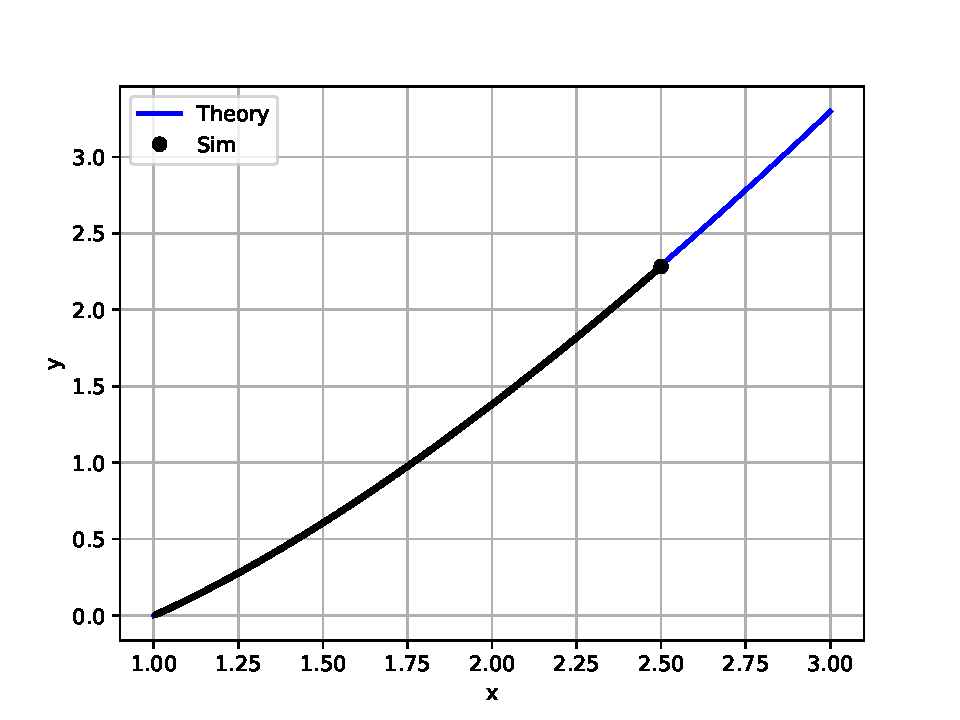
\includegraphics[width=\columnwidth]{figs/fig.pdf}
\end{figure}

I'm taking the initial conditions as $x=1$, $y=0$ and $h=0.006$. We compute the values of $x_n$ and $y_n$ using above recurrence relation. These values can be used to approximate the solution numerically for a given range of $x$.

\end{document}
